\documentclass[sans]{beamer}

\mode<presentation>
{
	% \usetheme{CambridgeUS}
	% \usetheme{Hannover}
	\usetheme{Singapore}
	\usecolortheme{default}
}

\usepackage{cmap}
\usepackage{listings}
\usepackage{lmodern}
\usepackage{color}
\usepackage{minted}
\usepackage{graphicx}
\usepackage{tikz}
\usetikzlibrary{arrows}
\usepackage{wrapfig}
\usepackage{bussproofs}
\usepackage{stmaryrd}

\usepackage[labelformat=empty]{caption}
\usepackage{fontspec}
% \usepackage{polyglossia}
% \setdefaultlanguage{russian}

% \setmainfont[Ligatures=TeX]{DejaVu Serif}
% \setsansfont[Ligatures=TeX]{DejaVu Sans}
% \setmonofont{DejaVu Sans Mono}

\definecolor{myGray}{RGB}{50,50,50}
\EnableBpAbbreviations

\begin{document}

\title
[Intuitionistic Logic]
{Intuitionistic Logic}

\subtitle{Based on S\o rensen, Urzyczyn lectures}

\author
[Podkopaev]{Anton Podkopaev, podkoav239@gmail.com}
\institute{JetBrains Lab}
\date [20-10-14]{20 oct 2014}

\begin{frame}[plain]
	\titlepage
\end{frame}

\begin{frame}{History}
  \begin{columns}

  \begin{column}{0.5\linewidth}
    \textbf{Luitzen Egbertus Jan Brouwer} (1881-1966)

    \vfill

    "Intuitionism" against Hilbert's "formalism"
  \end{column}

  \begin{column}{0.5\linewidth}
    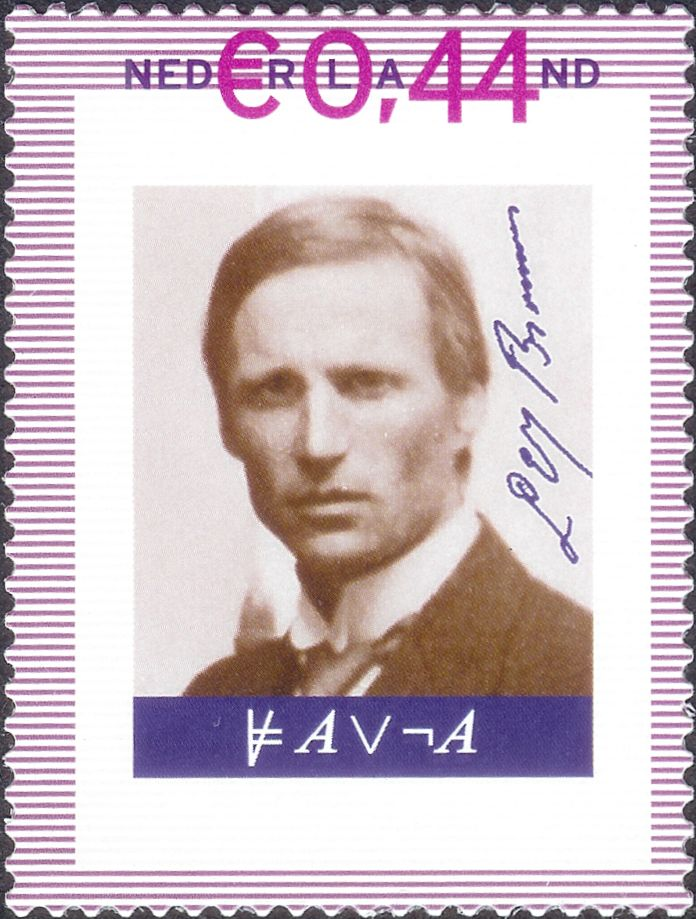
\includegraphics[width = \linewidth]{images/brouwer.jpg}
  \end{column}

  \end{columns}
\end{frame}

\begin{frame}{Example (1)}
  \emph{Tertium non datur:} $p \vee \lnot p$
  \pause
  \vfill
  \emph{
    There is seven $7$'s in a row somewhere in
    the decimal representation
    of the number $\pi$
  }
\end{frame}

\begin{frame}{Example (2)}
  \emph{
    There are two irrational numbers $x$ and $y$, such that $x^y$ is rational
  }
  \vfill
  \begin{block}{Proof:}
    if $\sqrt{2}^{\sqrt{2}}$ is a rational then we can take $x = y = \sqrt{2}$;

    otherwise take $x = \sqrt{2}^{\sqrt{2}}$ and $y = \sqrt{2}$
  \end{block}
\end{frame}

\begin{frame}{Intuitive semantics}
  \emph{BHK-interpretation} (for Brouwler, Heyting, Kolmogorov)

  \begin{block}{Rules:}
    \begin{itemize}
      \item A construction of $\varphi_1 \wedge \varphi_2$ consists of
            a construction of $\varphi_1$ and a construction of $\varphi_2$
      \item A construction of $\varphi_1 \vee \varphi_2$ consists of a
            number $i \in \{1, 2\}$ and a construction of $\varphi_i$
      \item A construction of $\varphi_1 \to \varphi_2$ is a method (function)
            transforming every construction of $\varphi_1$ into a construction
            of $\varphi_2$
      \item There is no possible construction of $\bot$ (where $\bot$ denotes falsity)
    \end{itemize}
  \end{block}
\end{frame}

\begin{frame}{Negation}
  Negation $\lnot \varphi$ is best understood as an abbreviation of an implication $\varphi \to \bot$

  \begin{itemize}
    \item A construction of $\lnot \varphi$ is a method that turns every construction of
      $\varphi$ into a non-existed object
  \end{itemize}
\end{frame}

\begin{frame}{Classic tautologies}
   \begin{enumerate}
     \item $\bot \to p$
     \item $((p \to q) \to p) \to p$
     \item $p \to \lnot \lnot p$
     \item $\lnot \lnot p \to p$
     \item $\lnot \lnot \lnot p \to \lnot p$
     \item $(\lnot q \to \lnot p) \to (p \to q)$
     \item $(p \to q) \to (\lnot q \to \lnot p)$
     \item $\lnot (p \wedge q) \to (\lnot p \vee \lnot q)$
     \item $(\lnot p \vee \lnot q) \to \lnot (p \wedge q)$
     \item $((p \leftrightarrow q) \leftrightarrow r) \leftrightarrow (p \leftrightarrow (q \leftrightarrow r))$
     \item $((p \wedge q) \to r) \leftrightarrow (p \to (q \to r))$
     \item $(p \to q) \leftrightarrow (\lnot p \vee q)$
     \item $\lnot\lnot (p \vee \lnot p)$
   \end{enumerate}
\end{frame}

\begin{frame}{Classic tautologies}
   \begin{enumerate}
     \item $\bot \to p$
     \item \textcolor{red}{$((p \to q) \to p) \to p$}
     \item $p \to \lnot \lnot p$
     \item \textcolor{red}{$\lnot \lnot p \to p$}
     \item $\lnot \lnot \lnot p \to \lnot p$
     \item \textcolor{red}{$(\lnot q \to \lnot p) \to (p \to q)$}
     \item $(p \to q) \to (\lnot q \to \lnot p)$
     \item \textcolor{red}{$\lnot (p \wedge q) \to (\lnot p \vee \lnot q)$}
     \item $(\lnot p \vee \lnot q) \to \lnot (p \wedge q)$
     \item \textcolor{red}{$((p \leftrightarrow q) \leftrightarrow r) \leftrightarrow (p \leftrightarrow (q \leftrightarrow r))$}
     \item $((p \wedge q) \to r) \leftrightarrow (p \to (q \to r))$
     \item \textcolor{red}{$(p \to q) \leftrightarrow (\lnot p \vee q)$}
     \item $\lnot\lnot (p \vee \lnot p)$
   \end{enumerate}
\end{frame}

\begin{frame}{Example of failure. $\lnot \lnot p \to p$}
  $\lnot \lnot p \to p = ((p \to \bot) \to \bot) \to p$

  \vspace{1cm}

  You need to construct $p$ from something that takes $p \to \bot$
  and returns $\bot$
\end{frame}

\begin{frame}{The language of logic}
  $\Phi ::= \bot \; | \; PV \; | \; (\Phi \to \Phi) \; |
   \; (\Phi \vee \Phi) \; | \; (\Phi \wedge \Phi) $

  \begin{itemize}
    \item $\lnot \varphi = \varphi \to \bot$
    \item $\varphi \leftrightarrow \psi = (\varphi \to \psi) \wedge (\psi \to \varphi)$
    \item The implication is right associative
  \end{itemize}
\end{frame}


\begin{frame}{Intuitionistic propositional calculus}
  \begin{prooftree}
    \AXC{$\Gamma, \varphi \vdash \varphi$ (Ax)}
  \end{prooftree}

  \begin{columns}
  
  \begin{column}{0.3\linewidth}
  \begin{prooftree}
    \AXC{$\Gamma \vdash \varphi$}
    \AXC{$\Gamma \vdash \psi$}
    \RightLabel{($\bigwedge$ I)}
    \BIC{$\Gamma \vdash \varphi \wedge \psi$}
  \end{prooftree}

  \begin{prooftree}
    \AXC{$\Gamma \vdash \varphi \wedge \psi$}
    \RightLabel{($\bigwedge$ E1)}
    \UIC{$\Gamma \vdash \varphi$}
  \end{prooftree}
  \begin{prooftree}
    \AXC{$\Gamma \vdash \varphi \wedge \psi$}
    \RightLabel{($\bigwedge$ E2)}
    \UIC{$\Gamma \vdash \psi$}
  \end{prooftree}
  \end{column}

  \begin{column}{0.3\linewidth}
  \begin{prooftree}
    \AXC{$\Gamma \vdash \varphi$}
    \RightLabel{($\bigvee$ I1)}
    \UIC{$\Gamma \vdash \varphi \vee \psi$}
  \end{prooftree}
  \begin{prooftree}
    \AXC{$\Gamma \vdash \psi$}
    \RightLabel{($\bigvee$ I2)}
    \UIC{$\Gamma \vdash \varphi \vee \psi$}
  \end{prooftree}
  \end{column}
 
  \begin{column}{0.4\linewidth}
  \begin{prooftree}
    \AXC{$\Gamma, \; \varphi \vdash \psi$}
    \RightLabel{($\to$ I)}
    \UIC{$\Gamma \vdash \varphi \to \psi$}
  \end{prooftree}
  \begin{prooftree}
    \AXC{$\Gamma, \; \varphi$}
    \AXC{$\Gamma \vdash \varphi \to \psi$}
    \RightLabel{($\to$ E)}
    \BIC{$\Gamma, \; \psi$}
  \end{prooftree}

  \begin{prooftree}
    \AXC{$\Gamma \vdash \bot$}
    \RightLabel{($\bot$ E)}
    \UIC{$\Gamma \vdash \varphi$}
  \end{prooftree}
  \end{column} 

  \end{columns}

  \begin{prooftree}
    \AXC{$\Gamma, \; \varphi \vdash \rho$}
    \AXC{$\Gamma, \; \psi \vdash \rho$}
    \AXC{$\Gamma \vdash \varphi \vee \psi$}
    \RightLabel{($\bigvee$ E)}
    \TIC{$\Gamma \vdash \rho$}
  \end{prooftree}
\end{frame}

\newcommand{\vsem}[1]{\llbracket #1 \rrbracket_v}
\newcommand{\vmsem}[1]{$\llbracket #1 \rrbracket_v$}
\newcommand{\got}[1]{$\mathbb{#1}$}
\newcommand{\gotb}{\got{B}}
\newcommand{\cali}[1]{$\mathcal{#1} \;$}
\newcommand{\calr}{\cali{R}}

\begin{frame}{The Boolean semantics}
  \begin{itemize}
    \item A \emph{valuation in} \gotb $\,$ is a map \emph{PV} $\to$ \gotb;
      such a map will also be called a 0-1 \emph{valuation}

    \vfill

    \item The map \vmsem{\bullet} : $\Phi \to$ \gotb $\,$ by:

      $\begin{aligned}
        \vsem{p} &= v(p) & for \; p \in PV \\
        \vsem{\bot} &= 0 \\
        \vsem{\varphi \vee \psi} &= max\{\vsem{\varphi}, \vsem{\psi}\} \\
        \vsem{\varphi \wedge \psi} &= min\{\vsem{\varphi}, \vsem{\psi}\}\\
        \vsem{\varphi \to \psi} &= max\{1 - \vsem{\varphi}, \vsem{\psi}\}
       \end{aligned}$

    \vfill
    \item We also write $v(\varphi)$ for \vmsem{\varphi}

    \vfill
  \item A formula $\varphi \in \Phi$ is a \emph{tautology} if $v(\varphi) = 1$ for
        all valuations in \gotb
  \end{itemize}
\end{frame}

\begin{frame}{The set-theoretic semantics}
  \begin{itemize}
    \item A \emph{field of sets (over X)} is a nonempty family \calr
      of subsets of $X$, closed under unions, intersections and complement (to $X$)
    
    \item \{\}, X $\in \mathcal{R}$
    
    \item A \emph{valuation in} \calr is a map $v: PV \to$ \calr
      
    \vfill

    \item The map \vmsem{\bullet} : $\Phi \to \mathcal{R}$ by:

      $\begin{aligned}
        \vsem{p} &= v(p) & for \; p \in PV \\
        \vsem{\bot} &= \{\} \\
        \vsem{\varphi \vee \psi} &= \vsem{\varphi} \cup \vsem{\psi} \\
        \vsem{\varphi \wedge \psi} &= \vsem{\varphi} \cap \vsem{\psi}\\
        \vsem{\varphi \to \psi} &= (X - \vsem{\varphi}) \cup \vsem{\psi}
       \end{aligned}$
  \end{itemize}
\end{frame}

\begin{frame}{Equivalence}
  The above two approaches to semantics are equivalent, i.e., the following conditions
  are equivalent for each field of subsets \calr over a nonempty set $X$:
  \begin{enumerate}
    \item $\varphi$ \emph{is a tautology}
    \item $v(\varphi) \,=\, X$, for all valuations $v \; in \; $\calr
  \end{enumerate}
\end{frame}

\begin{frame}{Boolean algebra}
  A \emph{Boolean algebra} is an algebraic system of the form
  $\mathcal{B} = \langle B, \cup, \cap, -, 0, 1\rangle$, where:
  \begin{itemize}
    \item $\cup, \cap$ are associative and commutative
    \item $(a \cup b) \cap c = (a \cap c) \cup (b \cap c) \;$ and
          $\; (a \cap b) \cup c = (a \cup c) \cap (b \cup c)$
    \item $a \cup 0 = a \;$ and $\; a \cap 1 = a$
    \item $-a \cup a = 1 \;$ and $\; -a \cap a = 0\;$
  \end{itemize}

  \vfill
  
  The relation $\leq$ defined as by $a \leq b$ iff $a \cup b = b$ is a partial order,
  $\cap, \cup$ are the \emph{glb} and \emph{lub} operations
\end{frame} 

\newcommand{\eqc}[1]{[#1]_{\sim}}
\newcommand{\mlg}{\mathcal{L}_{\Gamma}\;}
\newcommand{\mlgm}{$\mlg$}

\begin{frame}{Lindenbaum algebra}
  \begin{itemize}
    \item $\Gamma \subseteq \Phi$
    \pause
    \item $\varphi \sim \psi$ iff $\Gamma \vdash \varphi \to \psi$ and $\Gamma \vdash \psi \to \varphi$
    \pause
    \item $\mathcal{L} _{\Gamma} = {\Phi}/_{\sim} = \{\eqc{\varphi} : \varphi \in \Phi\}$
    \pause
    \item $\eqc{\varphi} \leq \eqc{\psi}$ iff $\Gamma \vdash \varphi \to \psi$
    \pause
    \item Operations over $\mathcal{L}_{\Gamma}$:

      $\begin{aligned}
        \eqc{\alpha} \cup \eqc{\beta} &= \eqc{\alpha \vee \beta}; \\
        \eqc{\alpha} \cap \eqc{\beta} &= \eqc{\alpha \wedge \beta}; \\
                     -\eqc{\alpha} &= \eqc{\lnot \alpha}
       \end{aligned}$
  \end{itemize}
\end{frame}

\begin{frame}{\mlgm properties}
  \begin{itemize}
    \item $\eqc{\bot}$ is the least element 0 of \mlgm
    \item $\eqc{\top}$ is the top element 1 of \mlgm
    
    \vfill
    \item $-a \cap a = \eqc{\bot}$
    \item \textcolor{red}{Not necessarily true:} $-a \cup a = \eqc{\top}$
    \vfill

    \item $c = (a \Rightarrow b)$ iff $c$ is the greatest element such that $a \cap c = b$
    \item $\eqc{\varphi} \Rightarrow \eqc{\psi} = \eqc{\varphi \to \psi}$

  \end{itemize}
\end{frame}

\begin{frame}{Heyting algebra}
  $\mathcal{H} = \langle H, \cup, \cap, \Rightarrow, -, 0, 1 \rangle$
  \begin{itemize}
    \item $\cup, \cap$ are associative and commutative
    \item $(a \cup b) \cap c = (a \cap c) \cup (b \cap c) \;$ and
          $\; (a \cap b) \cup c = (a \cup c) \cap (b \cup c)$
    \item $a \cup 0 = a \;$ and $\; a \cap 1 = a$
    \item $a \cup a = a$
    \item $a \cap c \leq b$ is equivalent to $c \leq a \Rightarrow b$,
      
      where $a \leq b$ stands for $a \cup b = b$

    \item $-a = a \Rightarrow 0$

    \vfill
    \pause
    
    \hrule
    \vfill

    \item Equals to a distributive lattice with zero and relative pseudo-complement defined
          for each pair of elements
    \item Each Boolean algebra is a Heyting algebra with $a \Rightarrow b = -a \cup b$

  \end{itemize}
\end{frame}

\begin{frame}{Non-Boolean example}
  $\mathcal{H} = \langle \mathcal{O}(\mathbb{R}^2), \cup, \cap, \Rightarrow, {\sim}, 0, 1 \rangle$
  \begin{itemize}
    \item $\mathcal{O}(\mathbb{R}^2)$ is the family of all open subsets 
    \item $A \Rightarrow B := Int(-A \cup B)$
    \item $0 = \{\}$ and $1 = \mathbb{R}^2$
    \item ${\sim} A = Int(-A)$
  \end{itemize}
\end{frame}

\begin{frame}{Heyting semantics for intuitionistic logic}
  \begin{itemize}
    \item A \emph{valuation v} in a \cali{H} is a map $v$ : \emph{PV} $\to$ \emph{H}
    \item The map \vmsem{\bullet} : $\Phi \to H$ by:

      $\begin{aligned}
        \vsem{p} &= v(p) & for \; p \in PV \\
        \vsem{\bot} &= 0 \\
        \vsem{\varphi \vee \psi} &= \vsem{\varphi} \cup \vsem{\psi} \\
        \vsem{\varphi \wedge \psi} &= \vsem{\varphi} \cap \vsem{\psi}\\
        \vsem{\varphi \to \psi} &= \vsem{\varphi} \Rightarrow \vsem{\psi}
       \end{aligned}$
  \end{itemize}
\end{frame}


\newcommand{\calh}{\cali{H}}
\newcommand{\mcalh}{\mathcal{H}}

\begin{frame}{Intuitionistical derivation rules}
  $\mathcal{H} = \langle H, \cup, \cap, \Rightarrow, {\sim}, 0, 1 \rangle$
  \begin{itemize}
    \item $\mcalh, v \models \varphi$, whenever $v(\varphi) = 1$
    \item $\mcalh \models \varphi$, whenever $\mcalh, v \models \varphi$, for all $v$
    \item $\mcalh, v \models \Gamma$, whenever $\mcalh, v \models \varphi$, forall $\varphi \in \Gamma$
    \item $\mcalh \models \Gamma$, whenever $\mcalh, v \models \Gamma$, forall $v$
    \item $\models \varphi$, whenever $\mcalh, v \models \varphi$, for all $H, v$
    \item $\Gamma \models \varphi$, whenever $\mcalh, v \models \Gamma$ implies $\mcalh, v \models \varphi$, for all $H$ and $v$
  \end{itemize}

  \vfill
  $\models \varphi$ means that $\varphi$ is \emph{intuitionistically valid}, or \emph{intuitionistically tautology}

\end{frame}

\begin{frame}{Equivalence}
  \textbf{Theorem.} \emph{Soundness and Completeness}
  
  The following conditions are equivalent:
  \begin{enumerate}
    \item $\Gamma \vdash \varphi$
    \item $\Gamma \models \varphi$
  \end{enumerate}

  \vfill
  \pause
  \textbf{Example.}
  
  Peirce's law $((p \to q) \to p) \to p$ isn't intuitionistically valid

\end{frame}

\begin{frame}{Properties}
  \emph{Intuitionistic logic isn't finite-valued:}

  There is no single finite Heyting algebra \calh such that $\vdash \varphi$ is equivalent to
  $\mcalh \models \varphi$

  \pause
  \vfill
  \textbf{Theorem}
  \begin{enumerate}
    \item A formula $\varphi$ of length $n$ is valid iff it is valid in all Heyting algebras
          of cardinality at most $2^{2^n}$
    \item Let \calh be the algebra of all open subsets of a dense-in-itself metric space $V$.
          Then $\mcalh \models \varphi$ iff $\varphi$ is valid
  \end{enumerate}

\end{frame}

\begin{frame}{Kripke model}
  A \emph{Kripke model} --- $\mathcal{C} = \langle C,\leq,{\Vdash} \rangle$
  \begin{itemize}
    \item $C$ --- a non-empty set
    \item $\leq$ --- a partial order on $C$
    \item $\Vdash$ --- a relation between $C$ and \textbf{propositional variables}
    \begin{itemize}
      \item If $c \leq c'$ and $c \Vdash p$ then $c' \Vdash p$
    \end{itemize}
  \end{itemize}
\end{frame}

\begin{frame}{$\Vdash$ generalization to $\Phi$}
  A \emph{Kripke model} --- $\mathcal{C} = \langle C,\leq,{\Vdash} \rangle$
  \begin{itemize}
    \item $c \Vdash \varphi \vee \psi$ iff $c \Vdash \varphi$ or $c \Vdash \psi$
    \item $c \Vdash \varphi \wedge \psi$ iff $c \Vdash \varphi$ and $c \Vdash \psi$
    \item $c \Vdash \varphi \to \psi$ iff $c' \Vdash \psi$, for all $c'$ such that $c \leq c'$ and $c' \Vdash \varphi$
    \item $c \Vdash \bot$ never happens

    \vfill
    \pause
    \item $c \Vdash \lnot \varphi$ iff $c' \nVdash \varphi$, for all $c' \geq c$
  \end{itemize}

  \pause
  \vfill
  This definition preserves:
  \begin{itemize}
      \item If $c \leq c'$ and $c \Vdash \varphi$ then $c' \Vdash \varphi$
  \end{itemize}
\end{frame}

\begin{frame}{Filter}
  A \emph{filter} in a Heyting algebra $\mcalh \langle H, \cup, \cap, \Rightarrow, -, 0, 1\rangle$ is a nonempty subset $F$ of $H$, such that
  \begin{itemize}
    \item $a, b \in F$ implies $a \cap b \in F$
    \item $a \in F$ and $a \leq b$ implies $b \in F$
  \end{itemize}

  \vfill
  A filter $F$ is \emph{proper} iff $F \neq H$
  \vfill
  A proper filter $F$ is \emph{prime} iff $a \cup b \in F$ implies that either $a$ or $b$ belongs to $F$
\end{frame}

\begin{frame}{Properties}
  \textbf{Lemma}

  $F$ --- proper filter in $\mathcal{H}$, $a \notin F$. There exists a prime filter $G$ such that $F \subseteq G$ and $a \notin G$
  \vfill

  \pause
  \textbf{Lemma}

  $v$ --- a valuation in $\mathcal{H}$. There is $\mathcal{C} = \langle C, \leq, \Vdash \rangle$,
  such that $\mcalh, v \models \varphi$ iff $\mathcal{C} \Vdash \varphi$, for all formulas $\varphi$
  
  \vfill

  \pause
  \textbf{Theorem}

  The sequent $\Gamma \vdash \varphi$ is provable iff for all Kripke models $\mathcal{C}$, the condition
  $\mathcal{C} \Vdash \Gamma$ implies $\mathcal{C} \Vdash \varphi$

\end{frame}

\begin{frame}{The implicational fragment}
  \textbf{Theorem}

  The implicational fragment of intuitionistic propositional calculus is complete
  with respect to Kripke models, i.e., $\Gamma \vdash \varphi$ is provable iff for all Kripke
  models $\mathcal{C}$, the condition $\mathcal{C} \Vdash \Gamma$ implies $\mathcal{C} \Vdash \varphi$
  
  \vfill

  \pause
  \textbf{Theorem}

  $\varphi$ --- implicational formula. $\Gamma$ --- set of implicational formulas.

  If $\Gamma \vdash \varphi$ can be derived in the intuitionistic propositional calculus then
  it can be derived in the implicational fragment
\end{frame}

\end{document}
